\documentclass[xetex,mathserif,serif]{beamer}
\usepackage{polyglossia}
\setdefaultlanguage[babelshorthands=true]{russian}
\usepackage{minted}
\usepackage{tabu}

\useoutertheme{infolines}

\usepackage{fontspec}
\setmainfont{FreeSans}
\newfontfamily{\russianfonttt}{FreeSans}

\definecolor{links}{HTML}{2A1B81}
\hypersetup{colorlinks,linkcolor=,urlcolor=links}

\setbeamertemplate{blocks}[rounded][shadow=false]

\setbeamercolor*{block title alerted}{fg=red!50!black,bg=red!20}
\setbeamercolor*{block body alerted}{fg=black,bg=red!10}

\tabulinesep=1.2mm

\title{Code review}
\author[Юрий Литвинов]{Юрий Литвинов\\\small{\textcolor{gray}{yurii.litvinov@gmail.com}}}
\date{10.04.2018г}

\newcommand{\todo}[1] {
	\begin{center}\textcolor{red}{TODO: #1}\end{center}
}

\newcommand{\attribution}[1] {
\vspace{-5mm}\begin{flushright}\begin{scriptsize}\textcolor{gray}{\textcopyright\, #1}\end{scriptsize}\end{flushright}
}

\begin{document}

	\frame{\titlepage}

	\begin{frame}
		\frametitle{Доклады}
		\begin{itemize}
			\item Обзор платформы .NET Core
			\item Тестирование пользовательского интерфейса, Coded UI и White
			\item yield return, ленивые вычисления
			\item Обзор библиотеки Unity
			\item Обзор технологии Silverlight
		\end{itemize}
	\end{frame}

	\begin{frame}
		\frametitle{Code Review, что это такое}
		\begin{columns}
			\begin{column}{0.5\textwidth}
				\begin{itemize}
					\item Проверка кода ``глазами''
					\item Повышение качества ПО и квалификации программистов
					\item Обнаруживаются ошибки, которые не поймать тестированием:
					\begin{itemize}
						\item Плохая архитектура
						\item Плохое оформление
						\item Уязвимости к атакам
						\item Утечки памяти
						\item Проблемы с производительностью
					\end{itemize}
				\end{itemize}
			\end{column}
			\begin{column}{0.5\textwidth}
				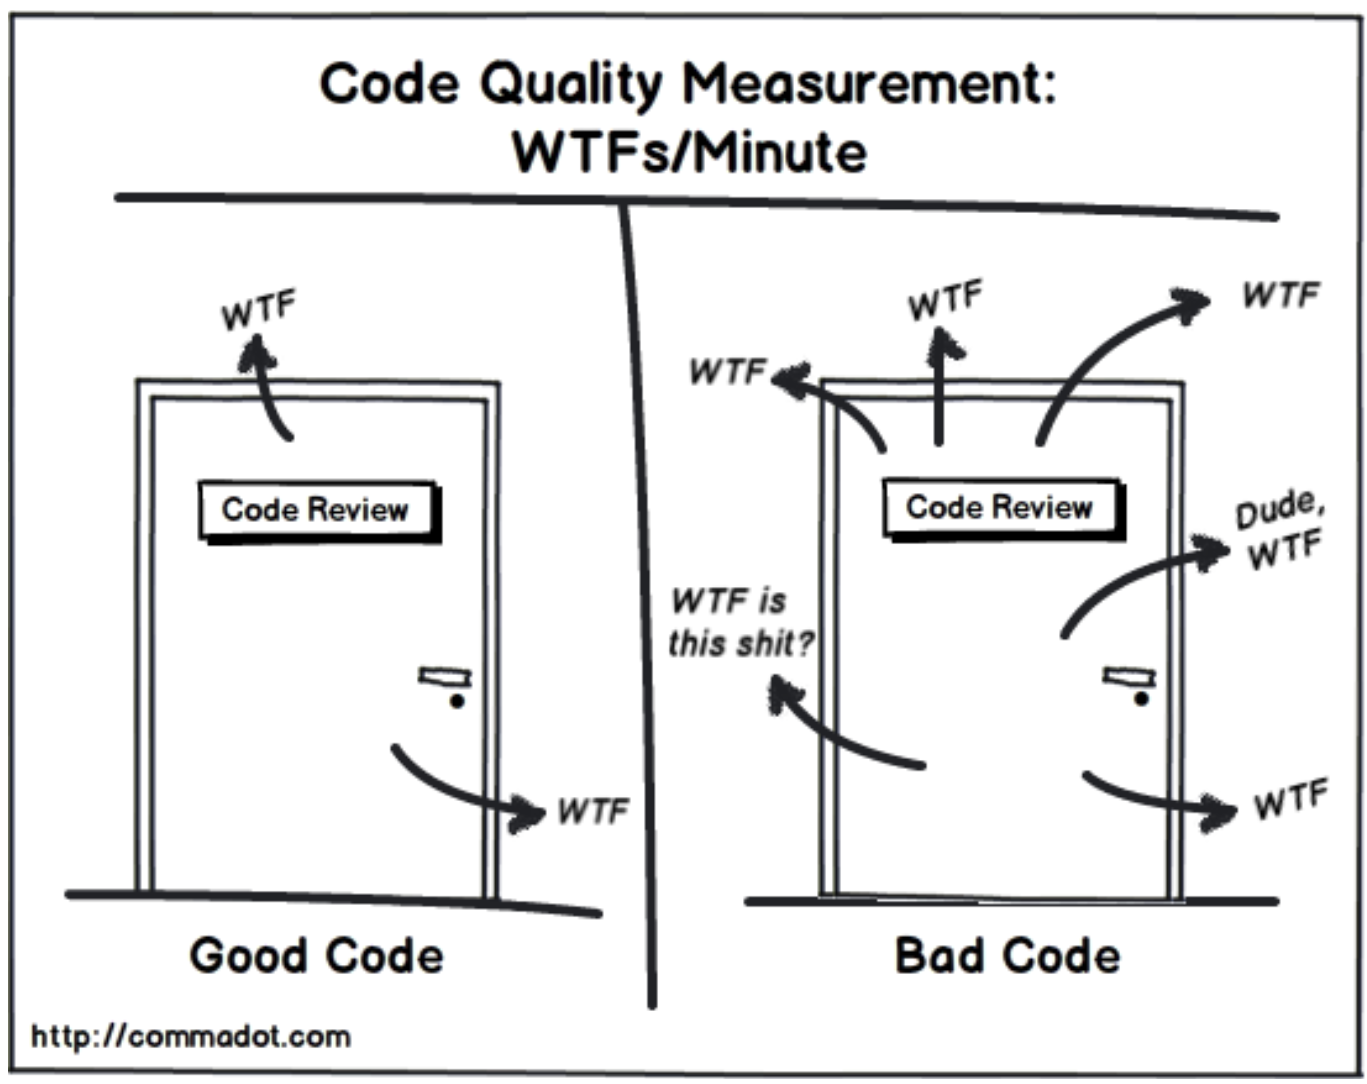
\includegraphics[width=0.9\textwidth]{wtfs.png}
			\end{column}
		\end{columns}
	\end{frame}

	\begin{frame}
		\frametitle{Правила проведения}
		\begin{itemize}
			\item Формальные и неформальные ревью
			\begin{itemize}
				\item Часто код не принимается без ревью в основную ветку
				\item Иногда выбирают случайный кусок кода, рассылают его заранее всем участникам ревью, после чего собираются для обсуждения
			\end{itemize}
			\item Код безличен, обсуждается не автор, а код
			\begin{itemize}
				\item Общее владение кодом
			\end{itemize}
			\item Не только указываются ошибки, но и пути исправления
		\end{itemize}
	\end{frame}

\end{document}
